\chapter{Review of Literature }
\section{Literature Survey}
We have gone through various evaluation and grading tools as per our observation there are not single system which is been made for both android and website.The creation of rubrics system is very tedious and unclear to the user.The application are only targeted for certain events which is the biggest drawback.\\
There are hardly any feedback system that has been provided by this application system.Hence following is the summary that we have inferred from our research\\
\begin{figure}[H]
\centering
\hfill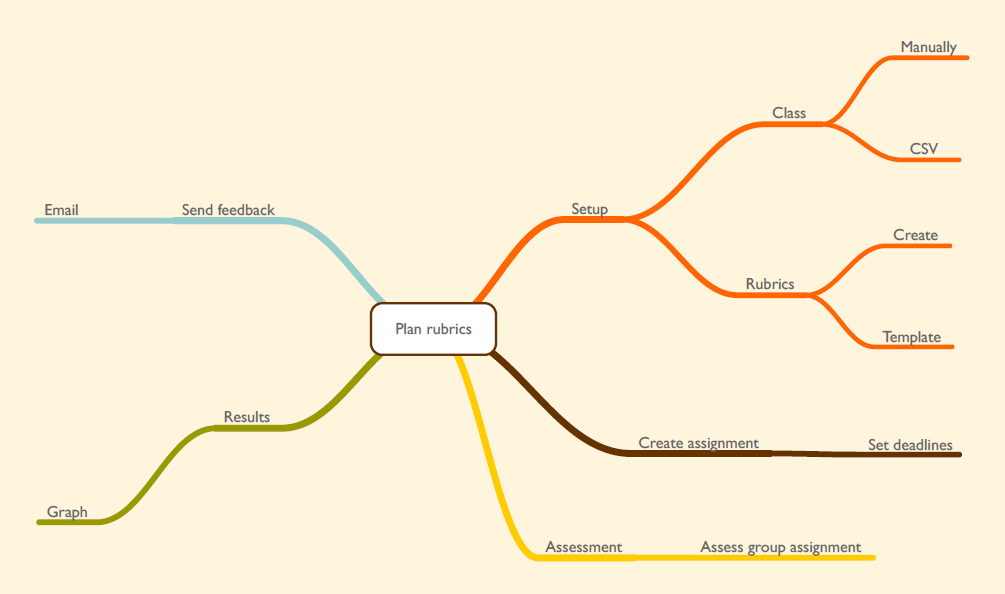
\includegraphics[scale=0.6]{project/images/mindmap}\hspace*{\fill}
\caption{Rubrics System}
\end{figure}
\newpage
{Comparison done between the tools / methods / algorithms}
\begin{table}[H]
\centering
\begin{tabular}{|l|l|l|l|l|l|}
\hline
\textbf{Features}                                                         & \textbf{Rubistar} & \textbf{Moodle} & \textbf{iRubrics} & \textbf{EssayTagger} & \textbf{Rubric System} \\ \hline
Multiple Template                                                         & Yes               & No              & No                & No                   & Yes                    \\ \hline
\begin{tabular}[c]{@{}l@{}}Dynamically create\\ template\end{tabular}     & Yes               & Yes             & Yes               & No                   & Yes                    \\ \hline
\begin{tabular}[c]{@{}l@{}}Graphical performance \\ analysis\end{tabular} & No                & Yes             & No                & No                   & Yes                    \\ \hline
User Convenient                                                           & Yes               & No              & No                & Yes                  & Yes                    \\ \hline
Cost                                                                      & Yes               & Yes             & Yes               & Yes                  & No                     \\ \hline
Feedback to student                                                       & No                & Yes             & Yes               & Yes                  & Yes                    \\ \hline
\end{tabular}
\caption{Comparison Between the tools}
\label{my-label}
\end{table}